\documentclass[17pt, fleqn]{beamer}
\usepackage{default}
\usetheme{default}
% Copenhagen, Madrid would also be possibilities.
% \setbeamercovered{transparent}

\usepackage[utf8]{inputenc}
\usepackage[T1]{fontenc}
\usepackage{amsmath,amssymb,lmodern}

\usepackage{tikzit}
\input{presentation_style_file.tikzstyles}
\graphicspath{{graphics/}}

\title[]{Masterarbeit}
\author[]{Daniel Siemmeister}
\date[]{2022 - 07 - 07}

% begin document
\begin{document}

\begin{frame}[plain]
    \titlepage    
\end{frame}

\begin{frame}{Titel der Arbeit}
\centering
\large{Erprobung unterschiedlicher Machine Learning Ansätze für die Vorhersage der Prüfungsaktivität von Studierenden}
\end{frame}

\begin{frame}
    Wie viele prüfungsaktive Studierende gibt es in drei Jahren? \\[1cm]
    \pause
    Ansätze des LQM \\[1cm]
    \pause
    Prädiktion der Wahrscheinlichkeit, in drei Jahren prüfungsaktiv zu sein - ohne konkrete Klassifizierung
\end{frame}

\begin{frame}{Machine Learning}
    \small{
    $ \mathcal{X} \dots \text{Menge der Inputdaten} $ \\[0.2cm]
    $ \mathcal{Y} \dots \text{Menge der Outputdaten} $ \\[0.2cm]
    $ \mathcal{D_{\mathbf{X}}} \dots \text{Verteilung über } \mathcal{X} $ \\[0.2cm]
    $ f(\cdot) \dots \text{mit } Y = f(\mathbf{X}) + \epsilon $ \\[0.2cm]
    $ S = \{ (\mathbf{x}_1, y_1), \dots , (\mathbf{x}_n, y_n) \} \text{ mit n Datenpunkten} $ \\[0.2cm]
    $ \mathcal{D} \dots \text{gemeinsame Verteilung von } (\mathbf{X}, Y) $ \\[0.2cm]
    }
\end{frame}

\begin{frame}{Machine Learning}
    \small{
    $ \mathcal{H} = \{ h( \cdot, \mathbf{w}) | \mathbf{w} \in \mathbf{W} \} $ \\[0.2cm]
    $ \mathcal{A} \dots \text{Algorithmus mit } h_S = \mathcal{A}(S) $ \\[0.2cm]
    $ l : \mathcal{H} \times \mathcal{Z} \rightarrow \mathbb{R}_+ \dots \text{loss-Funktion, wobei } \mathcal{Z} = \mathcal{X} \times \mathcal{Y} $ \\[0.2cm]
    $ L_D(\mathcal{A}) = \mathbb{E}[l(\mathcal{A}(S), (\mathbf{X}, Y)) ] \dots \text{wahre Risikofunktion} $ \\[0.2cm]
    $ L_S(h_S) = \frac{1}{n} \sum_{i=1}^n l(h_S, (\mathbf{x}_i, y_i)) \dots \text{empirische Risikofunktion} $ \\[0.2cm]
    }
\end{frame}

\begin{frame}{Machine Learning}
    \small{
        mit $ \epsilon $ wird Verteilung von $ \mathcal{D}_{Y|\mathbf{X}} $ festgelgt \\ [0.2cm]
        Parameter von $ \mathcal{D}_{Y|\mathbf{X}} $ soll mittels $ h_S $ approximiert werden \\ [0.2cm]
        Sinvolle Wahlen: Erwartungswert, Median \\ [0.2cm]
        loss-Funktion entscheidet darüber, welcher Parameter approximiert wird
        \begin{itemize}
            \item $l(h_S, (\mathbf{X}, Y)) = (Y - h_S(\mathbf{X}))^2 $ approximiert $\mathbb{E}[Y|\mathbf{X}] $
            \item $l(h_S, (\mathbf{X}, Y)) = |Y- h_S(\mathbf{X})| $ approximiert $m(Y|\mathbf{X}) $ (Median) 
        \end{itemize}
    }
\end{frame}

\begin{frame}{Machine Learning}
    \small{
        erwarteter Output: $ \bar{y}(\mathbf{x}) = \mathbb{E}[Y|\mathbf{X} = \mathbf{x}] $ \\[0.5cm]
        erwartete Vorhersagefunktion: $ \bar{h} = \mathbb{E}[\mathcal{A}(S)] = \int_{\mathbb{R}^{(d+1)n}} h_s p_S(s)  \,ds $ \\[0.5cm]
        $ \mathcal{L}_{\mathcal{D}}(\mathcal{A}) = \mathbb{E}[(h_S(\mathbf{\mathbf{X}})-Y)^2] $ wird zu \\[0.5cm]
        \footnotesize{$ \underbrace{\mathbb{E}[(h_S(\mathbf{X})- \bar{h}(\mathbf{X}))^2]}_{\text{Variance}}+\underbrace{\mathbb{E}[(\bar{h}(\mathbf{X})-\bar{y}(\mathbf{X}))^2]}_{\text{Bias}^2} + \underbrace{\mathbb{E}[(\bar{y}(\mathbf{X})-Y)^2]}_{\text{Noise}} $
    }}
    
\end{frame}


\begin{frame}{Problemstellung}
    \begin{tiny}
		\tikzfig{problemstellung}
	\end{tiny}
    
\end{frame}

\begin{frame}{Relevanz der Problemstellung}
    \begin{figure}
        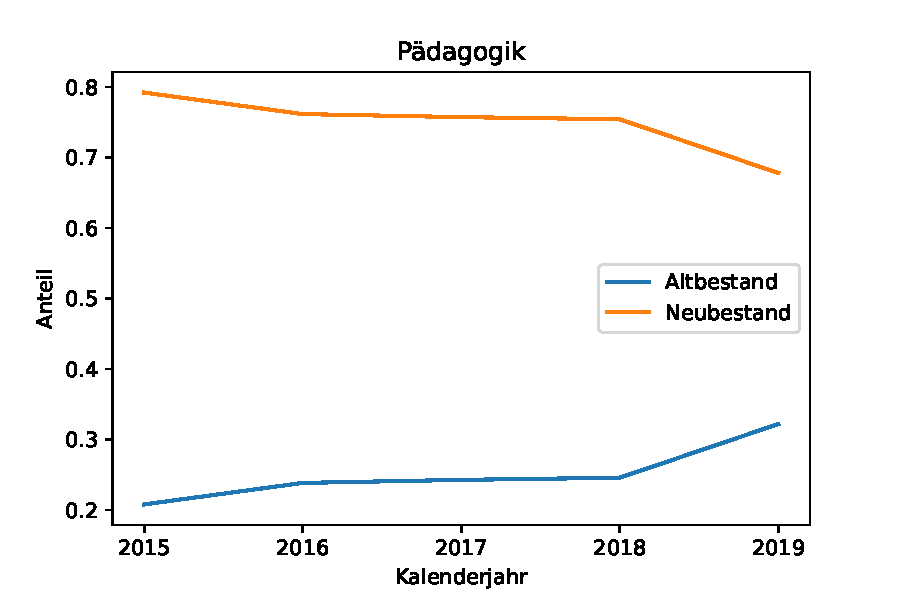
\includegraphics[width = 0.5\columnwidth]{pad2.pdf}
        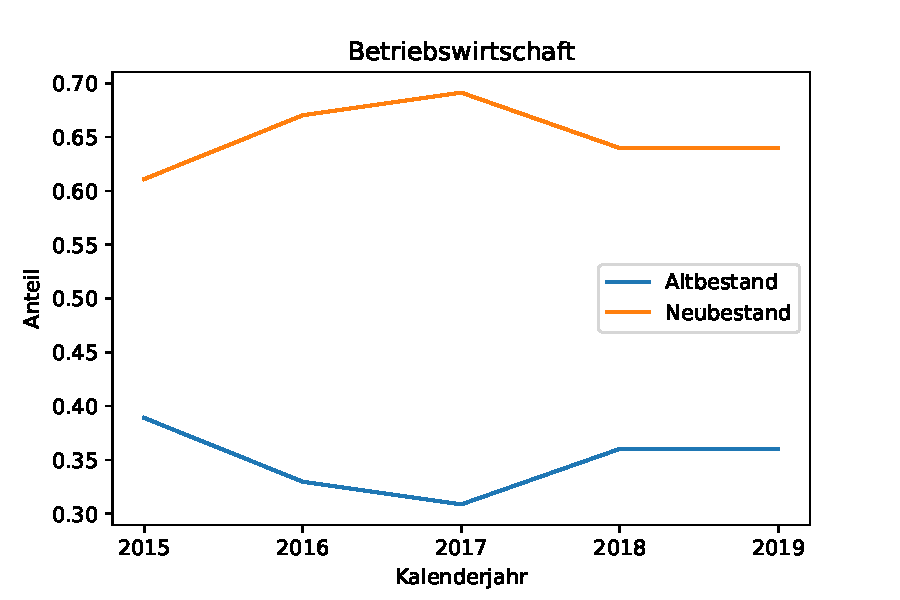
\includegraphics[width = 0.5\columnwidth]{bwl2.pdf}
        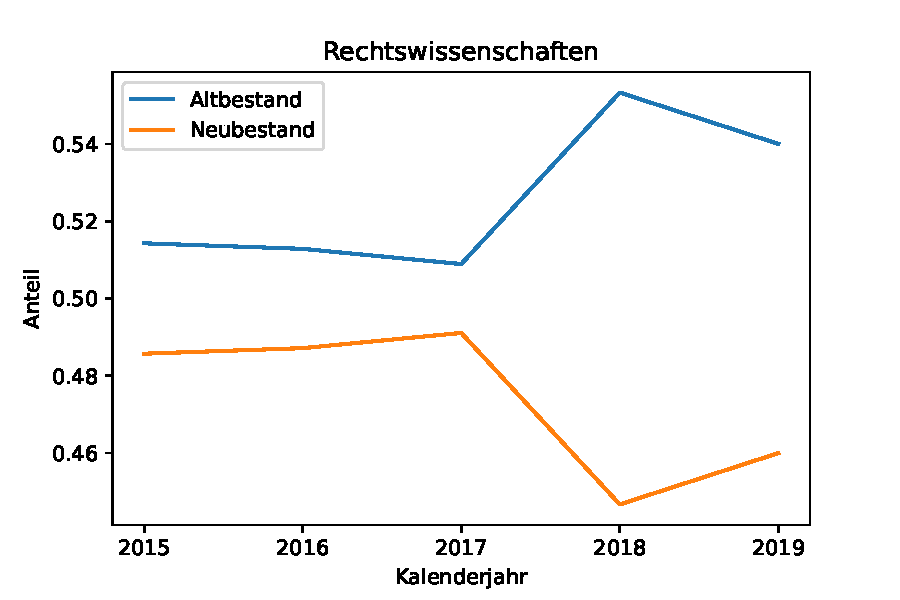
\includegraphics[width = 0.5\columnwidth]{jus2.pdf}
        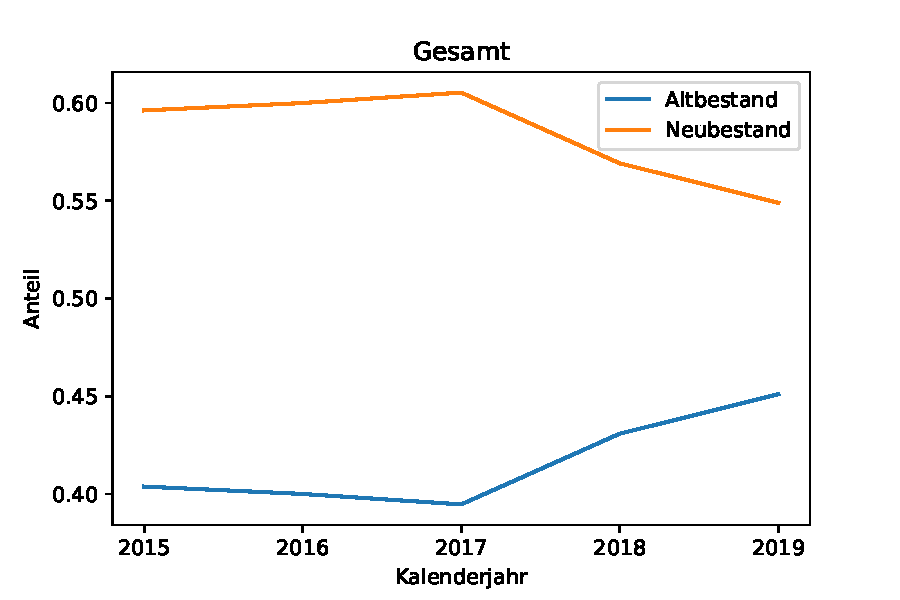
\includegraphics[width = 0.5\columnwidth]{ges2.pdf}
    \end{figure}
    
\end{frame}

\begin{frame}
    Problem 1: \\
    Schätzung der prüfungsaktiven Studierenden, von den bereits Anzahl und Merkmalskombinationen vorhanden sind \\[1cm]

    \pause

    Problem 2: \\
    Schätzung der prüfungsaktiven Studierenden, von denen weder Anzahl noch Merkmalskombinationen vorhanden sind    
\end{frame}

\begin{frame}{Herangehensweise Problem 1}
    \begin{itemize}
        \item Regression der ECTS \\[1cm]
        \pause
        \item Markov Ketten Modell \\[1cm]
        \pause
        \item Schätzung der Wahrscheinlichkeit aktiv zu sein, ohne zu klassifizieren
    \end{itemize}
    
\end{frame}

\begin{frame}{Ergebnisse für Problem 1}
    \begin{itemize}
        \item[X]
        \item[X]
        \item[\checkmark] 
    \end{itemize}

    
\end{frame}

\begin{frame}{Herangehensweise Problem 2}
    \begin{itemize}
        \item Schätzung der Anzahl der Studierenden mit gleicher Merkmalskombination wie im Jahr zuvor \\[1cm]
        \pause
        \item Clustering der Studierenden und anschließende Schätzung der Anzahl nach Cluster
    \end{itemize}
    
\end{frame}

\begin{frame}{Ergebnisse für Problem 2}
    \begin{itemize}
        \item[$\sim$]
        \item[$\sim$] 
    \end{itemize}
    
\end{frame}

\begin{frame}{Beiträge}
    Klare Darstellung der Problemstellung \\[1cm]
    \pause
    Erprobung unterschiedlicher Ansätze \\[1cm]
    \pause
    Machine Learning Ansatz für Problem 1, der gute Ergebnisse liefert \\[1cm]
    \pause
    Notwendigkeit von mehr Daten, um Ansätze weiter zu Erproben
    
\end{frame}






\end{document}